\section{Blockschaltbild des Projekts}\label{sec:3.1}
Nach einigen Überlegungen über die beste Herangehensweise an dieses Projekt, wurde folgendes Blockschaltbild entwickelt:
\begin{figure} [H]
	\centering
	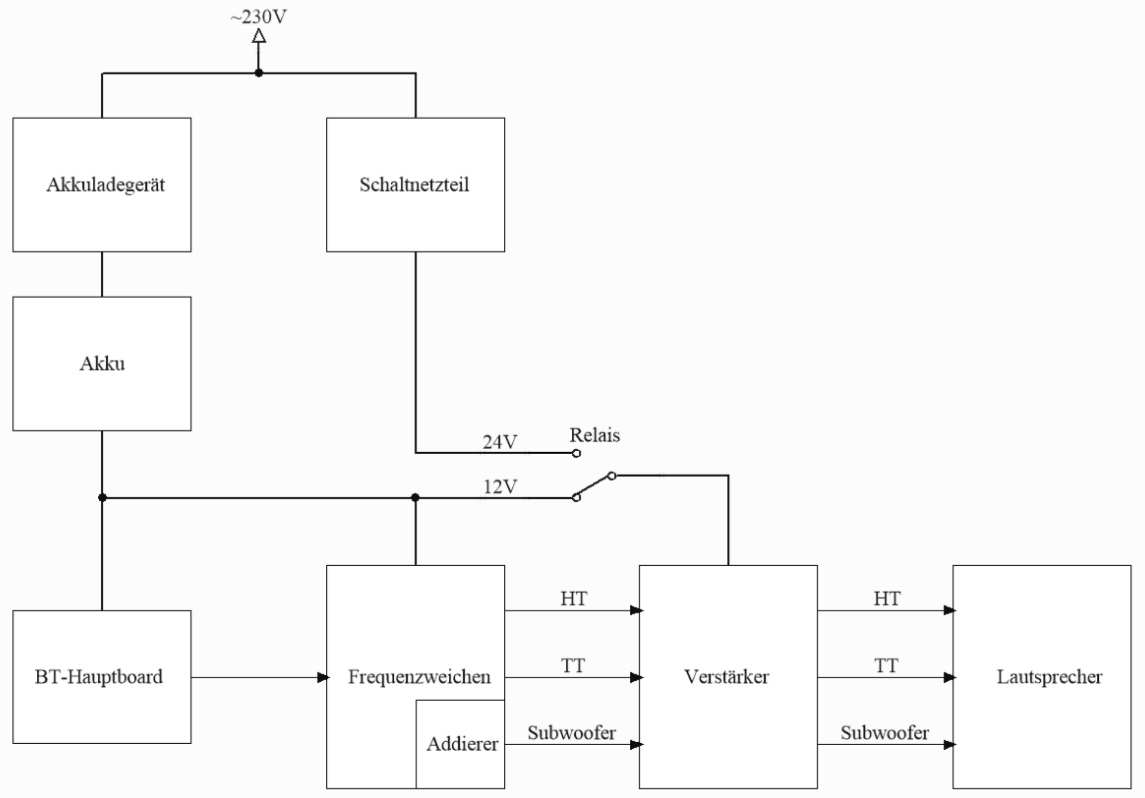
\includegraphics[width=1\textwidth]{img/blockschaltbild.png}
	\caption{Blockschaltbild}
	\label{fig:3.1.1}
\end{figure}
Ein wichtiger Teil des Projekts ist die Bluetooth-Hauptplatine (in Abb. \ref{fig:3.1.1} links unten).
Diese Platine ist der Eingang der Schaltung.
Das Stereo-Audio-Signal kann mithilfe der BT-Hauptplatine mittels Klinkenbuchse oder Übertragung über Bluetooth (siehe: Kap. \ref{sec:3.3}) ins System eingespeist werden.
\\ \\
Dieses Signal wird dann mithilfe der Frequenzweichen in 3 verschiedene Frequenzbereiche, Hochton-, Mitte-Tiefton- und Bassbereich, aufgetrennt.
Ab diesem Zeitpunkt existieren dann 3 verschiedene Stereo-Signale im System und müssen auch unabhängig voneinander weiterverarbeitet werden.
\\
Der Addierer innerhalb der Frequenzweichen hat die Aufgabe, das Stereo-Signal in ein Mono-Signal umzuwandeln (weitere Erklärung: Kap. \ref{sec:3.2}).
\\
Insgesamt gibt es dann also 5 Signale, die weiterverarbeitet werden.
\\ \\
Die verschiedenen Audio-Signale werden dann mit je einem Verstärker auf einen angemessenen Pegel verstärkt.
Nach diesem Vorgang wird jedes Audio-Signal an seinen passenden Lautsprecher geleitet.
Die 2 Hochton-Signale für linken und rechten Kanal werden an die entsprechenden Hochton-Lautsprecher weitergeleitet.
Das gleiche passiert auch mit den beiden Mitte-Tiefton-Signalen.
Übrig bleibt das Mono-Signal für den Bassbereich.
Es wird an den einzelnen Subwoofer geleitet.
\\ \\
Versorgt wird die Elektronik mit 12 V oder 24 V, genauere Erklärung im Kapitel \ref{sec:3.4}.

\newpage
\section{Mehrweg-Lautsprechersysteme}\label{sec:3.2}
Ein Lautsprecher ist ein Bauelement, dass ein elektrisches Signal in ein akustisches Signal (20 Hz bis 20 kHz) umwandelt.
Dabei wird eine Membran in Schwingung versetzt, die wiederum die umgebende Luft zum Schwingen bringt und einen hörbaren Ton erzeugt.
\\ \\
Nun wird aber nicht jede Frequenz gleich gut von ein und demselben Lautsprecher abgestrahlt.
Durch die physikalischen Gegebenheiten strahlen große Membranen tiefe Frequenzen besser ab, als hohe Frequenzen.
Daher ist es sinnvoll, mehrere Lautsprecher für verschiedene Frequenzbereiche zu verwenden.
Benannt werden diese verschiedenen Lautsprecher durch den Bereich in dem sie am besten funktionieren.
Beispielsweise Hochton-Lautsprecher oder Hochtöner für den Hochton-Bereich (>2,5 kHz).
Wie gut nun verschiedene Frequenzen von einem Lautsprecher abgestrahlt werden, ist in seinem Frequenzgang ersichtlich:
\begin{figure} [H]
	\centering
	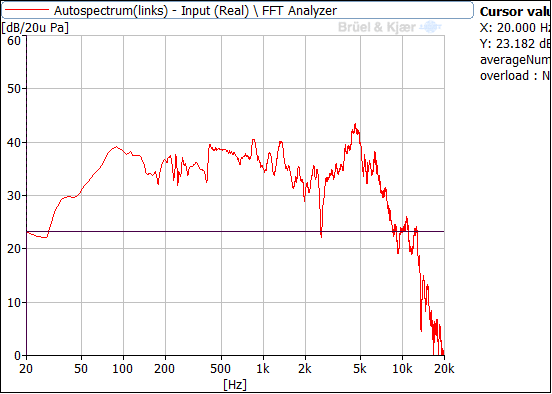
\includegraphics[width=1\textwidth]{img/LSMessung/TT1_9,17l_bestes.png}
	\caption{Beispiel eines Frequenzganges (Tieftöner PSS 297 58206)}
	\label{fig:3.2.1}
\end{figure}
Bei einem perfekten Lautsprecher würde diese Linie (Abb. \ref{fig:3.2.1}) eine parallele Gerade zur X-Achse bilden.
Da so ein Lautsprecher aber nicht existiert, werden verschiedene Frequenzen auch mit einem verschiedenen Schalldruckpegel vom Lautsprecher abgestrahlt.
\\
In dem Beispiel (Abb. \ref{fig:3.2.1}) wurde ein Tieftöner gemessen.
Das ist klar ersichtlich, da der Schalldruckpegel ab 5 kHz fast kontinuierlich fällt.
Tiefere Frequenzen werden, in einem gewissen Bereich, gleich wiedergegeben.
\\ \\
Je nach Frequenzbereich kann ein Ton vom menschlichen Ohr auch lokalisiert \mbox{werden}.
Hohe Frequenzen (<20 kHz) sind besser lokalisierbar als tiefe Frequenzen.
Bei sehr niedrigen Frequenzen (<150 Hz) ist der Ton gar nicht mehr lokalisierbar.
Diesen \mbox{Effekt} kann man nutzen und damit akustische Effekte erzeugen.
Einige Lautsprecher-Systeme, die diesen Effekt nutzen sind:
\begin{itemize}
	\item 2.0-System
	\item 2.1-System
	\item 5.1-System
\end{itemize}
Dabei steht die erste Zahl für die Anzahl der verteilten Lautsprecher und die zweite Zahl für die Anzahl der verwendeten Subwoofer.
\\
Je mehr verteilte Lautsprecher benutzt werden, desto bessere Raumklang-Effekte sind realisierbar.
Dadurch wird die Beschaltung aber auch komplizierter, da 5 verschiedene Audio-Signale verwendet werden.
\\ \\
Der Subwoofer ist ein spezieller Lautsprecher.
Er arbeitet im Bass-Bereich(20-150 Hz) und verarbeitet nur ein einziges Signal.
Diese Frequenzen sind nicht lokalisierbar, weshalb auch nur ein Subwoofer benötigt wird.
Meistens ist die Membran des Subwoofers um einiges größer als die Membran der anderen Lautsprecher.
Damit kann der Subwoofer mehr Luft in Bewegung setzen und somit einen höheren Schalldruckpegel erzeugen.
Um das zu ermöglichen benötigt der Subwoofer aber auch mehr Leistung als die anderen Lautsprecher.
\\ \\
In unserem Projekt haben wir uns direkt für ein 2.1-System entschieden, da sich dieses System am besten bewährt hat und für Musik ein Stereo-System völlig ausreicht.
Die zwei verteilten Boxen, auch Satelliten genannt, sind mit je einem Hochton- und einem Tiefton-Lautsprecher ausgestattet und werden über Kabeln mit der Hauptbox verbunden.
Damit sollen die Satelliten fast den gesamten Frequenzbereich für Audio (20 Hz bis 20 kHz) abdecken.
Der einzelne Subwoofer übernimmt den Bass-Bereich (<150 Hz) und sitzt in der Hauptbox.
Dort ist auch die gesamte Elektronik verbaut.

\section{Signalübertragung über Bluetooth}\label{sec:3.3}
Bluetooth ist eine moderne Funkschnittstelle für verschiedenste Anwendungen.
Unter anderem gibt es auch speziell für Audio-Anwendungen konzipierte Protokolle.
Die Übertragung läuft folgendermaßen ab:
\\
Zuerst muss das sendende Gerät (z.B. ein Smartphone) mit dem empfangenden Gerät (z.B. Bluetooth-Modul) verbunden werden.
Danach werden die gewünschten Daten ausgewählt.
In diesem Fall wären die Daten ein Musikstück.
Über Funk werden die digitalen Daten an das empfangende Gerät gesendet.
Nun muss das Bluetooth-Modul diese digitalen Daten wieder in ein analoges Signal umwandeln, welches dann weiterverarbeitet werden kann.
\\ \\
Dabei ist eine hohe Kompatibilität mit viele Geräten wichtig, weil es sehr viele verschiedene Versionen von Bluetooth gibt.
Da Bluetooth-Geräte meist abwärtskompatibel sind, ist es sinnvoll das Modul mit einer älteren BT-Version laufen zu lassen.
\\ \\
Nach ausführlicher Recherche wurde das Modul \enquote{XS3868} ausgewählt.
Der darauf verbaute Chip \enquote{OVC3860} von \enquote{OmniVision Technologies} hat sich bereits in vielen anderen Projekten bewährt, da er günstig ist und Funktionen wie \enquote{Play/Pause} bereitstellt.
\newpage
Im \enquote{OVC3860} (Abb. \ref {fig:3.3.1}) ist außer der Bluetooth-Verbindung auch noch ein Stereo-Audio-Prozessor verbaut.
Zusätzlich gibt es noch eine UART-Schnittstelle mithilfe man einige Einstellungen am Chip vornehmen kann.
Eine LiPo-Akku-Ladeschaltung ist ebenfalls vorhanden, wird aber in diesem Projekt nicht verwendet.
\\
Das Modul benötigt eine Versorgungsspannung von 3,3 V bis 4,2 V, wobei der Chip mit 1,8 V versorgt wird.
Diese Spannung (1,8 V) wird auf dem Modul erzeugt.
\\
Die verwendete BT-Version ist 2.0.
Einige GPIO-Pins sind auf das Modul herausgeführt um Funktionen wie \enquote{Play/Pause} zu ermöglichen.
Der Chip benötigt einen externen Speicher und eine Antenne (auf dem Modul) um ordnungsgemäß zu funktionieren.
\begin{figure} [H]
	\centering
	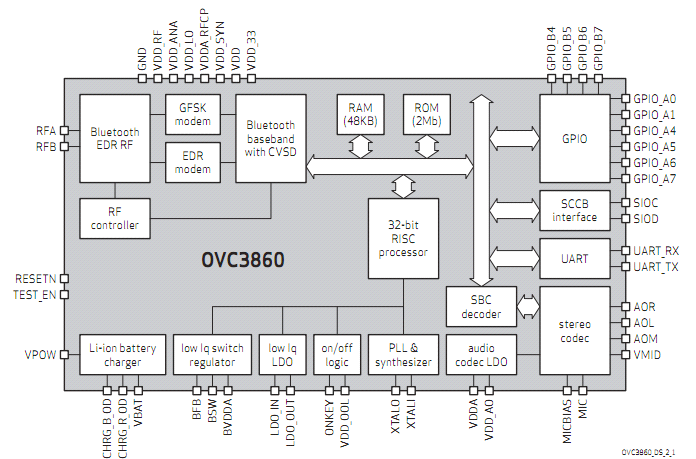
\includegraphics[width=1\textwidth]{img/BTModul/blockschaltbild.png}
	\caption[Blockschaltbild OVC3860]{Blockschaltbild OVC3860\footnotemark}\label {fig:3.3.1}
\end{figure}
\footnotetext{http://cxem.net/review/files/review24\_OVC3860.pdf,\\Zugriff: 11.03.2017}

\newpage
\section{Spannungsversorgung}\label{sec:3.4}
Da das Projekt portabel sein soll, ist auch ein Akku (Vlies-Blei-Akku) eingebaut.
Er versorgt die gesamte Elektronik mit 12 V bei Akkubetrieb.
Aufgeladen wird er durch ein passendes Ladegerät, welches aber nicht von uns entwickelt wird.
\\ \\
Falls eine externe Stromversorgung über eine Steckdose (230V AC) gegeben ist, ändert sich die Versorgung der Verstärker.
Während nun der Akku aufgeladen wird, schaltet ein Relais die Versorgungsspannung der Verstärker von 12 V auf 24 V um.
Diese Spannung (24 V) wird durch ein Schaltnetzteil erzeugt.
\\ \\
Durch eine höhere Spannung können die Verstärker auch die Signale auf höhere Spannungen verstärken.
Somit ergibt sich eine höhere Leistung an den Verstärkern aber auch an den Lautsprechern.
Eine Leistungssteigerung an einem Lautsprecher entspricht einer Steigerung des Schalldruckpegels was wiederum eine höhere Lautstärke bewirkt.
An den Verstärkern bewirkt eine höhere Leistung auch eine größere Wärmeentwicklung.
Der verbaute Kühlkörper muss diese Wärme bei Akkubetrieb als auch bei Netzbetrieb ableiten können.
\\ \\
Das Lautsprecher-System kann somit bei Netzbetrieb die Musik lauter abspielen als bei Akku-Betrieb.



